\documentclass[UTF8,a4paper,11pt]{ctexart}
\usepackage[margin=2.4cm]{geometry}
\usepackage{amsmath,amssymb,amsthm,booktabs,graphicx,placeins}
\usepackage[numbers,sort&compress]{natbib}
\usepackage{xurl}
\usepackage[hidelinks]{hyperref}
\newtheorem{theorem}{定理}
\newtheorem{proposition}[theorem]{命题}
\newtheorem{corollary}[theorem]{推论}
\allowdisplaybreaks
\setlength{\emergencystretch}{2em}
\renewcommand{\topfraction}{0.88}
\renewcommand{\bottomfraction}{0.66}
\renewcommand{\textfraction}{0.10}
\renewcommand{\floatpagefraction}{0.72}
\setcounter{totalnumber}{4}
\newcommand{\inner}[2]{\langle #1,#2\rangle}
\newcommand{\norm}[1]{\lVert #1\rVert}
\title{Muon有限步正交化的下降几何\\[0.3em]谱误差、方向曲率与训练收益}
\author{丁瀚洋}
\date{2026年11月}
\begin{document}
\maketitle
\begin{abstract}
Muon以有限步Newton--Schulz变换调整矩阵动量的奇异值。本文比较逐矩阵更新幅度相同时，
不同深度的极因子误差和目标下降收益。两个正定二次目标共享梯度、动量和Hessian特征值，
交换曲率方向即可反转候选的收益排序。这个反转在分别优化标量步长后仍然成立。
二维相图的5120个网格点均符合解析分界。
在WikiText103与TinyStories的36个Transformer更新前状态中，
加入方向曲率后，同批次收益差的平均绝对误差由0.08310降至0.00690 nats/token。
在独立批次的实际步长下，二阶预测和谱误差排序的一致率分别为94.4\%和96.3\%。
在26.5M参数的WikiText103配对实验中，深度从三步增至五步后，测试损失平均降低0.0847 nats/token。
三组语言建模设置中的目标反馈均以五步为主，平均测试损失比固定五步高0.0034至0.0046 nats/token。

\end{abstract}
\section{引言}
Muon对隐藏层矩阵的动量施加Newton--Schulz（NS）变换，再沿变换结果更新参数\cite{jordan2024muon}。
矩阵函数计算追求接近极因子，优化过程追求降低训练损失。
前者由动量矩阵的奇异值决定，后者还取决于当前梯度和目标曲率。
有限深度决定更新能量在奇异方向间的分配，并改变单步计算量。

已有研究从有限步NS的收敛性\cite{kim2026muonns,wang2026practical}、动量谱的规模规律\cite{magakyan2026spectral}和谱自适应计算\cite{topollai2026costfree}解释这一矩阵变换。
另一条研究线通过更新方向与曲率分析Muon的下降收益\cite{wang2026curvature}。
本文在同一训练位置比较有限NS候选的谱误差、梯度对齐和二阶下降量。
非衰减矩阵更新的均方根（RMS）与辅助优化设置保持一致，由此检验目标曲率如何改变候选排序，以及当次损失反馈能否改善深度选择。

为回答这个问题，本文首先构造具有相同梯度、相同动量和相同候选谱误差的一对二次目标。
两个目标只改变曲率，沿候选方向单独优化标量步长后，最佳方向仍发生反转。
对从有限集合在线选取深度的更新，本文给出统一的驻点收敛阶。
随后在真实训练检查点上生成完整参数更新，使用独立批次计算预测量和测量损失响应。
最后比较固定深度、目标反馈选择和训练阶段频率匹配的重放控制，将局部收益与完整训练轨迹联系起来。

曲率置换给出了候选排序发生反转的解析条件。在实际训练状态上，二阶项校正了低NS深度候选过高的一阶收益预测。
按谱误差排序在实际步长下同样准确。增大步长使五步候选在更多独立批次上取得最大下降，
从而把谱近似精度与训练收益的关系定位到具体的步长区间。


\section{相关工作}
谱范数约束下的最陡下降把矩阵梯度映射到其极因子，形成Muon的几何出发点\cite{bernstein2024norm}。
在大规模训练中，权重衰减和更新尺度是重要设计变量\cite{liu2025scalable}。
本文固定辅助优化器配置，并将每个隐藏矩阵的候选更新规范到相同RMS，从而单独考察谱形状。

有限NS理论刻画近似变换、动量和随机梯度如何影响驻点收敛\cite{kim2026muonns,wang2026practical,peng2026finitens}。
有限深度的平滑作用也进入了非光滑优化分析\cite{li2026smoothing}。
本文研究给定训练状态上的候选排序，以完整参数步长的下降量作为评价对象。

谱规模规律揭示了层类型和模型规模与NS输入谱之间的联系\cite{magakyan2026spectral}。
谱自适应方法利用Gram矩阵的矩估计谱分布，再选择近似程序\cite{topollai2026costfree}。
定向谱干预进一步研究不同奇异方向在训练中的作用\cite{goyal2026targeted}。
本文同时测量矩阵函数误差和目标响应，使用相同动量的曲率置换解释两种排序的差异。

曲率视角通过一阶下降和二阶代价分析Muon与Adam的差异\cite{wang2026curvature}。
本文用完整Hessian--向量积比较有限NS候选，保留跨层与辅助更新的交叉项。
线性预测和二阶预测在同一组独立批次上接受比较。阶段匹配重放用来衡量当次目标反馈的作用。

\section{幅度匹配的有限NS更新}\label{sec:v2method}
对隐藏层矩阵$W_\ell$，令当前批梯度为$G_{t,\ell}$，动量递推为
\begin{equation}
 B_{t,\ell}=\beta B_{t-1,\ell}+(1-\beta)G_{t,\ell},\qquad
 M_{t,\ell}=\beta B_{t,\ell}+(1-\beta)G_{t,\ell}.
\end{equation}
由$X_0=M/\norm{M}_F$出发，经验NS采用
\begin{equation}\label{eq:v2ns}
 X_{j+1}=3.4445X_j-4.7750(X_jX_j^{\mathsf T})X_j
              +2.0315(X_jX_j^{\mathsf T})^2X_j.
\end{equation}
记$Q_k(M)=X_k$，零矩阵的变换取零。经典三次NS采用$X_{j+1}=1.5X_j-0.5X_jX_j^{\mathsf T}X_j$，
精确极因子由紧致SVD计算。经验深度$k$作为干预变量，谱误差由实际输出测量。

设矩阵含$d_\ell$个元素。主对照使用
\begin{equation}\label{eq:v2rms}
 D_{k,\ell}=0.2\sqrt{d_\ell}\,
       \frac{Q_k(M_{t,\ell})}{\norm{Q_k(M_{t,\ell})}_F},
 \qquad \operatorname{RMS}(D_{k,\ell})=0.2.
\end{equation}
$M_{t,\ell}=0$时直接取$D_{k,\ell}=0$。
各深度使用相同动量、矩阵学习率、衰减和训练批次。
嵌入、输出与一维参数交给同一配置的AdamW\citep{loshchilov2019adamw}。输出头与词嵌入共享权重。
完整候选步长写成$S_k=\eta_t D_k+U_t$，其中$D_k$在辅助参数位置为零，$U_t$包含共享辅助更新及权重衰减。
参数按$w_{t+1}=w_t-S_k$更新。

幅度匹配动量直接规范化$M_{t,\ell}$，RMS-Adam则规范化AdamW的非衰减方向
$\widehat m/(\sqrt{\widehat v}+\epsilon)$。Moonlight尺度消融保留$Q_5$，
对$m_\ell\times n_\ell$矩阵取$D_{5,\ell}=0.2\sqrt{\max(m_\ell,n_\ell)}\,Q_5(M_{t,\ell})$\citep{liu2025scalable}。

对逐矩阵RMS相同的极因子$P_\ell$，定义归一化谱误差
\begin{equation}
 E_k^2=\frac{\sum_\ell\norm{D_{k,\ell}-P_\ell}_F^2}
                  {\sum_\ell\norm{P_\ell}_F^2}.
\end{equation}
同时记录动量的稳定秩、奇异值分位数和候选更新的梯度对齐。

\paragraph{独立批次的目标测量。}
梯度批次$A$生成完整候选，包括共享辅助更新。批次$B$用来计算
\begin{equation}\label{eq:v2scores}
 a_k=\inner{\nabla f_B(w)}{S_k},\qquad
 b_k=\inner{S_k}{\nabla^2f_B(w)S_k},\qquad
 \widehat\Delta_k=a_k-\tfrac12b_k.
\end{equation}
Hessian--向量积对完整参数向量求导，保留跨矩阵与辅助参数的交叉项。
另一批次$C$测量$\Delta_{C,k}=f_C(w)-f_C(w-S_k)$。
每次测量后恢复起点参数。各候选共享起点、数据和计算精度。

\paragraph{Probe-NS。}
每隔100次更新，Probe-NS从训练集另取4096个token，评价$k\in\{1,3,5\}$的完整候选，选择
\begin{equation}
 k_t=\operatorname*{arg\,min}_{k\in\{1,3,5\}} f_B(w-S_k).
\end{equation}
相同损失取较小深度，选定深度沿用到下一次探测。第一次探测前使用深度5。
阶段匹配重放将同一种子的选择点分成四段。存在不同排列的段从其他排列中均匀抽样，
最后一次选择保留原位，使各深度的实际更新次数与探测计算保持一致。
两者的差异衡量当次目标反馈相对于阶段频率安排的收益。

谱误差选择器Error-NS使用相同的候选集、学习率和选择周期，以$E_k$最小为准选择深度。
该策略用紧致SVD获得参考极因子，将矩阵函数的近似目标直接作为选择依据。
它与Probe-NS的配对比较考察两种评价目标带来的训练差异。

\section{下降几何与曲率反转}\label{sec:v2theory}
先研究一个正定二次目标。记$g=\nabla f(w)$，$H$为Hessian，对给定方向$D$定义
\begin{equation}\label{eq:v2gain}
 a(D)=\inner{g}{D},\quad b(D)=\inner{D}{H[D]},\quad
 \Delta(\eta,D)=\eta a(D)-\frac{\eta^2}{2}b(D).
\end{equation}
当$a(D),b(D)>0$时，沿该方向的最优步长与收益为
\begin{equation}\label{eq:v2optimal}
 \eta^*(D)=\frac{a(D)}{b(D)},\qquad
 J(D)=\frac{a(D)^2}{2b(D)}.
\end{equation}
$J(cD)=J(D)$对$c>0$成立，因此该指标消除了方向幅度与标量学习率的影响。
当$H=hI$且$h>0$时，Cauchy--Schwarz不等式给出
$J(D)\le\norm{g}^2/(2h)$，沿梯度方向取等。
因此在各向同性曲率下，更新收益由与真实梯度的夹角决定。
梯度与动量重合且奇异值平坦时，各深度归一化后沿同一个方向。

\begin{theorem}[相同动量下的曲率反转]\label{thm:v2reversal}
设$u,v$为线性无关的单位Frobenius方向，且$a_u=\inner{g}{u}>0$、$a_v=\inner{g}{v}>0$。
令$c=\inner{u}{v}$。对$0<\epsilon<1$定义
\begin{equation}
 H_u[X]=X-(1-\epsilon)\inner{X}{u}u,\qquad
 H_v[X]=X-(1-\epsilon)\inner{X}{v}v,
\end{equation}
以及$f_i(X)=\inner{g}{X}+\tfrac12\inner{X}{H_i[X]}$，$i\in\{u,v\}$。
两个目标在$X=0$的梯度相同，Hessian的最大特征值均为1、最小特征值均为$\epsilon$。
其方向收益满足
\begin{align}
 \frac{J_u(u)}{J_u(v)}&=\frac{a_u^2}{a_v^2}
       \frac{\epsilon+(1-\epsilon)(1-c^2)}{\epsilon},\\
 \frac{J_v(v)}{J_v(u)}&=\frac{a_v^2}{a_u^2}
       \frac{\epsilon+(1-\epsilon)(1-c^2)}{\epsilon}.
\end{align}
当$\epsilon$充分小时，$u$在$f_u$上更优，$v$在$f_v$上更优，两个收益比均按$\epsilon^{-1}$增长。
\end{theorem}
\begin{proof}
算子$H_u$在$u$方向上的特征值为$\epsilon$，在其正交补上的特征值为1。因此
\[
 \inner{u}{H_u[u]}=\epsilon,\qquad
 \inner{v}{H_u[v]}=1-(1-\epsilon)c^2
                =\epsilon+(1-\epsilon)(1-c^2).
\]
代入式\eqref{eq:v2optimal}得到第一个比值，交换$u,v$得到第二个比值。
由线性无关性，$1-c^2>0$，两比值在$\epsilon\to0$时均趋于无穷。
\end{proof}

取相同动量矩阵产生的两个有限NS方向为$u,v$，即可在整个构造中保持候选及其谱误差不变。
在相同RMS下逐方向优化步长后，曲率置换仍然改变收益排序。
接下来固定梯度和动量，交换曲率，检验候选排序和理论收益比。

\begin{corollary}[谱信息相同时的选择代价]\label{cor:v2selector}
考虑从$\{u,v\}$中选取方向的确定性规则，其输入由当前位置的梯度、动量、候选谱误差和Hessian特征值组成。
在定理\ref{thm:v2reversal}的两个目标上，该规则给出同一选择。
当$\epsilon$趋于零时，至少一个目标上所选方向与最优候选的收益比以$O(\epsilon)$趋于零。
\end{corollary}
\begin{proof}
两个目标的规则输入逐项相同。若规则选$u$，在目标$f_v$上取定理中第二个收益比的倒数。
若规则选$v$，在目标$f_u$上取第一个收益比的倒数。两个倒数均为$O(\epsilon)$。
\end{proof}

\begin{proposition}[二维谱方向的精确分界]\label{prop:v2boundary}
设$g=(1,\rho)$、$H=\operatorname{diag}(1,\kappa)$，其中$\rho,\kappa>0$。
比例为$r>0$的方向有收益
\[
 J(r)=\frac{(1+\rho r)^2}{2(1+\kappa r^2)}.
\]
对$r>s>0$，分界为
\begin{equation}\label{eq:v2boundary}
 \kappa_* =\frac{2\rho+\rho^2(r+s)}{r+s+2\rho rs}.
\end{equation}
$\kappa<\kappa_*$时$J(r)>J(s)$，$\kappa>\kappa_*$时排序相反。
连续方向比例的最优值为$r_*=\rho/\kappa$。
\end{proposition}
\begin{proof}
将$J(r)-J(s)$通分，其分子为
\[
 (r-s)\big[2\rho+(\rho^2-\kappa)(r+s)-2\rho\kappa rs\big].
\]
分母严格为正，解中括号为零得到式\eqref{eq:v2boundary}。
直接求导可得$J'(r)$的符号由$\rho-\kappa r$决定，得到$r_*$。
\end{proof}

\begin{proposition}[完整参数步长的局部预测]\label{prop:v2taylor}
设$f$的Hessian在线段$\{w-tS:0\le t\le1\}$上为$L_H$-Lipschitz。
对$a=\inner{\nabla f(w)}{S}$、$b=\inner{S}{\nabla^2f(w)S}$，有
\begin{equation}
 f(w)-f(w-S)=a-\tfrac12b+R(S),\qquad
 |R(S)|\le\frac{L_H}{6}\norm{S}^3.
\end{equation}
\end{proposition}
\begin{proof}
对$\phi(t)=f(w-tS)$应用二阶Taylor公式。
$|\phi''(t)-\phi''(0)|\le L_H t\norm{S}^3$，积分余项的绝对值至多为
$L_H\norm{S}^3\int_0^1t(1-t)\,dt=L_H\norm{S}^3/6$。
\end{proof}
式\eqref{eq:v2scores}给出该预测的可测版本。
线性项衡量梯度与完整更新的对齐，二阶项衡量目标沿该更新的曲率代价。
将$S_k=\eta D_k+U$代入二次型后，交叉项$2\eta\inner{D_k}{H[U]}$随候选变化。
因此测量完整步长也保留共享更新对排序的影响。
实验分别比较两者的排序能力，并用独立批次检验预测的迁移。

\subsection{任意有限深度选择下的驻点收敛}\label{sec:v2convergence}
沿用有限步分析中分离动量误差的思路\cite{wang2026practical,peng2026finitens}，
这里对所有候选使用同一个逐块幅度和对齐下界。
以下分析将参数写成矩阵块$w=(W_1,\ldots,W_L)$。内积及范数取各块的Frobenius直积。
设$f$有下界$f_*$，梯度为$L_f$-Lipschitz，且相对于历史$\mathcal F_t$，
批梯度$G_t$满足$\mathbb E[G_t\mid\mathcal F_t]=g_t=\nabla f(w_t)$和
$\mathbb E[\norm{G_t-g_t}^2\mid\mathcal F_t]\le\sigma^2$。
使用第\ref{sec:v2method}节的Nesterov动量，初始缓冲区为$B_{-1}=0$。
第$\ell$块的更新范数为$R_\ell>0$，深度从有限集合$\mathcal K$中选取，可依赖当前梯度和反馈批次。

令$q_k$为式\eqref{eq:v2ns}作用于奇异值的$k$步标量映射，
并定义
\[
 m=\min_{k\in\mathcal K,\ 0\le s\le1} q_k(s)/s,\qquad
 M=\max_{k\in\mathcal K,\ 0\le s\le1} q_k(s)/s,\qquad
 \alpha=m/M.
\]
$s=0$处采用连续延拓。因为$3.4445-4.7750 x+2.0315 x^2$的判别式为负且首项系数为正，
$q_k(s)/s$是紧集上的正连续函数，故$0<\alpha\le1$。
设$C=\alpha\min_\ell R_\ell$、$S=(\sum_\ell R_\ell^2)^{1/2}$，
选择$0\le\lambda\le C/[2(\norm{w_0}+\eta ST)]$，并记$S'=S+C/2$。

\begin{theorem}[幅度匹配有限NS的有限步界]\label{thm:v2convergence}
按$w_{t+1}=(1-\eta\lambda)w_t-\eta D_t$更新，
其中$D_t$由各块的幅度匹配NS方向组成。对$T\ge1$、$\eta>0$和$0\le\beta<1$，有
\begin{align}
 \frac1T\sum_{t=0}^{T-1}\mathbb E\norm{g_t}
 &\le \frac{2(f(w_0)-f_*)}{C\eta T}
     +\frac{L_f\eta (S')^2}{C} \nonumber\\
 &\quad+\frac{2(1+\alpha)S}{C}\left[
       \frac{\norm{g_0}}{T(1-\beta)}
       +\frac{L_f\eta S'}{1-\beta}
       +\sigma\sqrt{3(1-\beta)}\right].
\end{align}
取$\eta=c_1T^{-3/4}$和$1-\beta=c_2T^{-1/2}$，
其中$c_1>0$、$0<c_2\le1$，平均期望梯度范数为$O(T^{-1/4})$。
\end{theorem}

该界将各深度共享的方向下界与动量跟踪误差结合。
深度选择改变实际下降收益，同时保留同一个驻点收敛阶。证明见附录\ref{app:v2convergence}。

\section{实验设计}\label{sec:v2protocol}
\paragraph{精确几何与轨迹实验。}
二维实验独立扫描梯度比$\rho$和曲率比$\kappa$，在固定最大Hessian特征值1及共同更新RMS下比较各方向，
并沿每个方向优化标量步长。矩阵实验使用$16\times16$变量、10个配对种子，控制Hessian条件数、谱方向关系与梯度噪声。
同动量置换实验使用定理\ref{thm:v2reversal}的两个算子，逐项验证收益比和排序反转。
多步轨迹使用相同问题、初始化与噪声序列，分别筛选学习率，运行500步的余弦衰减。
梯度奇异值的对数跨度取$0,0.5,1,2$，正跨度加入固定种子的轻微扰动。
同一种子在各曲率设置中使用相同的梯度、噪声方向和随机正交基。

\paragraph{语料与模型。}
语言实验采用WikiText103\cite{merity2016wikitext}与TinyStories\cite{eldan2023tinystories}。
每个语料取固定修订版本的5000万GPT-2 BPE训练token，记录末加入结束符。
WikiText103沿用官方验证与测试划分。TinyStories将官方验证故事按内容哈希分为验证与测试两组。
模型为预归一化因果Transformer，使用GELU、学习式位置嵌入及共享输入输出权重，
上下文长度256，填充词表大小50304。
两个配置分别为4层、宽384、6头的26,499,840参数模型，和8层、宽512、8头的51,069,952参数模型。
其中隐藏矩阵参数分别为7,077,888和25,165,824。

\paragraph{训练与学习率选择。}
每次更新处理8192个token，由微批4、梯度累积8组成。前向与NS矩阵乘法采用bfloat16，参数及优化器状态采用float32。
全局梯度裁剪阈值为1，动量系数0.95，AdamW的$\beta=(0.9,0.95)$，稳定项$10^{-8}$。
二维参数权重衰减为0.1，一维参数衰减为零。辅助学习率为0.001。
学习率前10\%步数线性预热，再余弦衰减到峰值的10\%。

每个优化器族从$\{0.0003,0.001,0.003\}$开始，在种子101上运行400步。
边界最优时将该边界按3倍向外扩展，随后在种子102上确认前两名，以两种子的平均验证损失选择配置。
主实验的NS1、NS3、NS5、Probe-NS、Error-NS与重放使用NS5选定的矩阵学习率。
较长训练对照使用NS3与NS5各自在筛选阶段选定的学习率。
两个语料及两个模型配置各自执行对应优化器族的筛选。

\paragraph{主对照与扩展。}
主实验比较AdamW、幅度匹配动量、NS1、NS3、NS5、Probe-NS、阶段匹配重放及Error-NS。
幅度消融在AdamW的学习率下匹配Adam方向的RMS，在NS5的学习率下使用Moonlight尺度。
规模与语料扩展分别比较AdamW、NS5及Probe-NS。
各设置运行种子0、1、2。同一种子共享初始化及训练数据序列，主对照的方法顺序按种子轮转。
主训练运行1000次更新，处理8,192,000个token。较长训练运行2500次更新，处理20,480,000个token。

\paragraph{局部干预与评价。}
在第250、500和1000次更新提交前，保存基础模型、实际GPU候选及动量。
离线测量加载这些完整候选，以float32数学注意力后端计算Hessian--向量积。
批次$B$含1024个token，独立批次$C$含4096个token。每个检查点重复两组采样，
分别在$0.5,1,2$倍实际步长上比较预测与响应。
倍率作用于完整步长$S_k$，包括辅助参数和权重衰减分量。
精确极因子和经典三次NS作为参考。
记录的投影Hessian、梯度对齐、谱误差和候选损失组成可重放的局部几何数据。

训练每250步验证一次。WikiText103的验证覆盖完整分割，TinyStories使用固定262144个目标的验证前缀。
验证选择最佳检查点，再对完整测试分割计分。损失单位为nats/token，分块计分按目标数量加权。
统计以独立训练种子为单位，局部干预先在各训练运行内聚合，再比较预测器和方法的配对差异。

\paragraph{计时。}
实验在一张RTX 3070 Ti Laptop GPU（8\,GB显存）上运行。两个模型规格分别从冻结权重出发，
对各方法使用同一组训练输入，作4次预热后同步测量12步。
分别记录前向与反向、梯度裁剪，以及优化器计算和提交步长的时间。
策略选择步的计时包含生成候选和计算选择分数。完整训练的墙钟另计验证和锚点写盘。

\section{结果与机制分析}\label{sec:v2results}
\subsection{同一个动量可以对应相反的最优方向}
固定$M=\operatorname{diag}(1,0.08)$时，NS1和NS5的方向比例分别为0.387和1.372，
幅度匹配后的极因子误差分别为0.413和0.155。
图\ref{fig:v2geometry}(a)在每个位置为两个方向分别求最优标量步长，
以$J_5/J_1$呈现方向本身的收益差异。取$\rho=0.1$时，分界$\kappa_*=0.117$。
当弱梯度方向的曲率高于该分界，NS1在这一方向分配的更新更小，获得更高的下降收益。
二维相图的5120个网格点均符合命题\ref{prop:v2boundary}的排序预测。

\begin{figure}[htbp]\centering
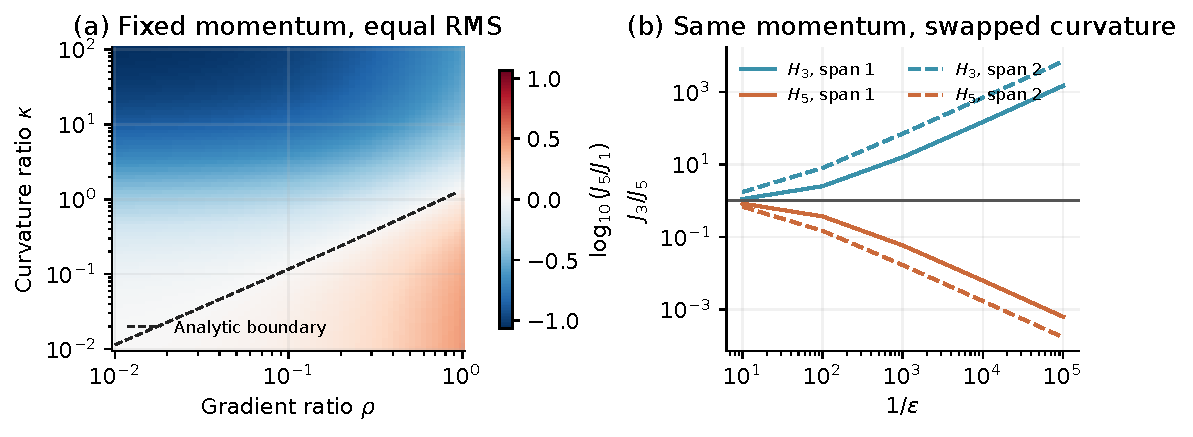
\includegraphics[width=\linewidth]{figures_v2/v2_geometry.pdf}
\caption{更新方向的收益分界。(a) 固定动量，改变梯度比$\rho$和曲率比$\kappa$。虚线为解析分界。
(b) 固定梯度与动量，分别沿NS3和NS5构造低曲率方向，绘出10个种子的几何平均收益比。}
\label{fig:v2geometry}
\end{figure}

在$16\times16$矩阵的曲率置换中，两个目标的Hessian特征值、初始梯度和候选谱误差逐项相同。
取$\epsilon=10^{-5}$，三个正谱跨度的30对目标全部反转NS3与NS5的排序。
将低曲率方向设置为NS3时，$J_3/J_5$的中位数为1947。置换为NS5时，$J_5/J_3$的中位数为1985。
该受控构造把收益差定位到方向与曲率的相对关系，差距随$1/\epsilon$增长，
与定理\ref{thm:v2reversal}的收益比一致。

\subsection{谱近似误差与优化收益采用不同的排序}
在更广泛的矩阵实验中，三种经验NS深度的更新幅度相同。
表\ref{tab:v2matrix}按梯度奇异值的对数跨度统计，极因子误差最小的候选在834个状态中的收益低于最优候选，
总计990个具有可区分收益的状态。
平坦谱、零噪声时三个方向重合，90个状态的收益并列。
图\ref{fig:v2errorgain}进一步比较固定条件数100下的两种曲率排列。
高曲率沿梯度主方向排列时，较平坦的更新谱可以减小曲率代价。
高曲率集中在尾部时，将更多更新能量分配给尾部会增加二阶代价。

\begin{table}[htbp]\centering
\caption{幅度匹配NS的谱误差和线优化收益。每个谱跨度含270个位置，来自10个配对种子。}
\label{tab:v2matrix}
\begin{tabular}{rrrr}
\toprule
对数谱跨度 & 非并列状态 & 误差最小候选收益次优 & 收益并列 \\ \midrule
0 & 180 & 97 & 90 \\
0.5 & 270 & 236 & 0 \\
1 & 270 & 237 & 0 \\
2 & 270 & 264 & 0 \\
\bottomrule
\end{tabular}

\end{table}

\begin{figure}[htbp]\centering
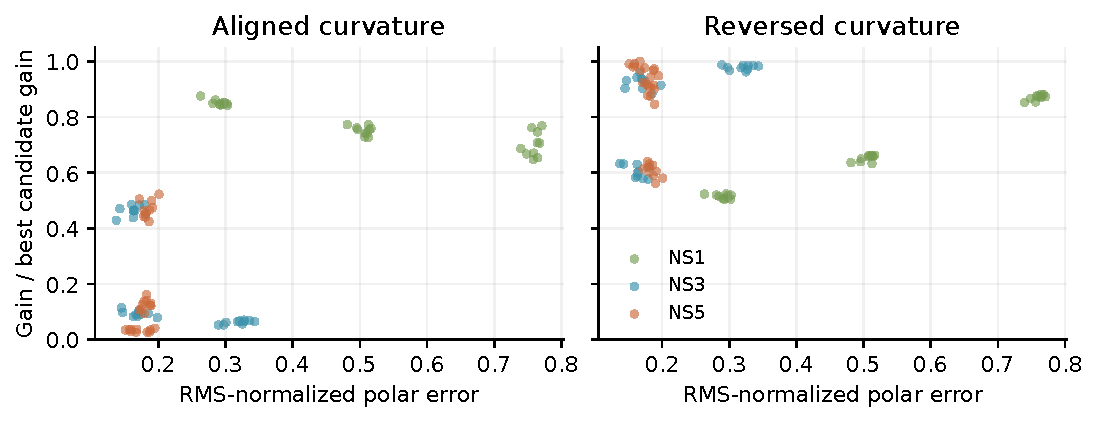
\includegraphics[width=\linewidth]{figures_v2/v2_error_gain.pdf}
\caption{条件数100、无噪声下的极因子误差与相对收益。正谱跨度及种子各自形成一个位置。
左图的低曲率沿梯度主方向排列，右图把高曲率移到梯度主方向。}
\label{fig:v2errorgain}
\end{figure}

分别选择学习率后，500步轨迹仍显示深度与噪声的交互。
在条件数100、倒置曲率的轨迹中，无噪声时NS3的终点目标均值为$7.20\times10^{-10}$，
低于NS5的$5.71\times10^{-9}$。
加入相当于初始梯度范数10\%的噪声后，幅度匹配动量的终点为$3.10\times10^{-4}$，
NS3和NS5则分别为$8.44\times10^{-4}$和$8.41\times10^{-4}$。
靠近最优点时真实梯度总体减小，固定尺度的噪声在观测梯度中占据更高比例。
谱变换改变观测谱中各方向的相对更新量，因而深度的作用随噪声条件变化。
完整轨迹与种子间变动见附录图\ref{fig:v2trajectory}。

\subsection{在冻结模型上测量方向曲率}
对同一个锚点，每个候选都从相同权重出发。比较任意两个候选$i,j$时，
用$\widehat\Delta_i-\widehat\Delta_j$预测它们的收益顺序。
给定共同的步长倍率$s$，一阶差为$s(a_i-a_j)$，二阶差再减去$s^2(b_i-b_j)/2$。
因此只改变步长倍率也可能改变排序。批次$B$与$C$分别提供预测和实测，
由此区分二阶式对当前目标的拟合与排序在数据上的迁移。
以三个经验深度为候选，预测器的成对一致率等于预测顺序与实测顺序一致的比例。
另设选择损失，定义为批次$C$上的最大候选下降量减去所选候选的下降量。
每个锚点内部完成所有候选配对，再以训练种子为单位聚合。

以主实验固定NS5、种子0的第250次更新为例，NS1与NS5的一阶下降预测分别为0.0652和0.0138。
NS1的二阶代价为0.1813，NS5为0.0077。将两个候选施加到独立批次$C$后，
NS1的损失上升0.1306，NS5的损失下降0.0037。
在这一位置，NS1沿梯度取得较大的一阶进展，但其方向上的曲率消耗了这份收益。

36个锚点共有72组独立批次测量。实际步长下，216个候选对在同一批次上的收益差平均绝对误差，
由一阶预测的0.08310降至二阶预测的0.00690 nats/token。
图\ref{fig:v2calibration}显示了这一改进。高曲率方向上的一阶预测明显偏高，二阶项校正了这部分差距。

\begin{figure}[htbp]\centering
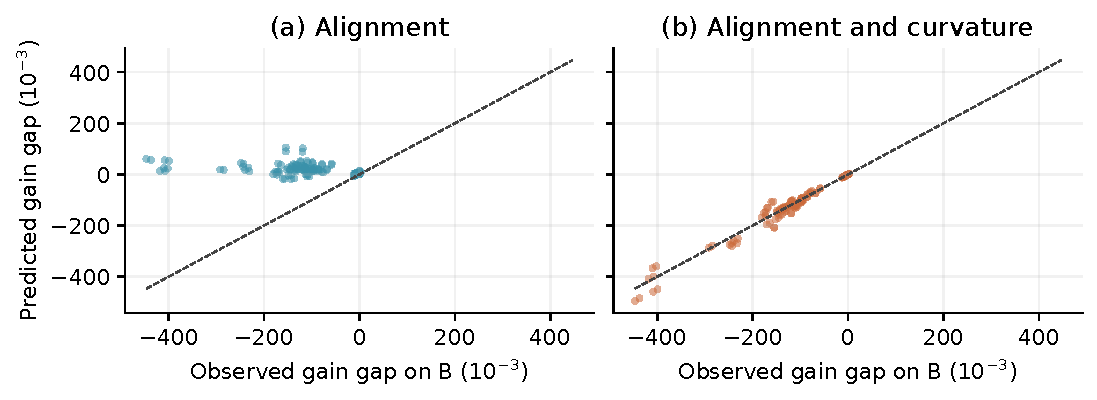
\includegraphics[width=\linewidth]{figures_v2/v2_curvature_calibration.pdf}
\caption{批次$B$上任意两个经验NS候选的下降量差。横轴为实际差值，纵轴为预测差值。虚线为两者相等。}
\label{fig:v2calibration}
\end{figure}

在独立批次$C$上，实际步长下的一阶排序一致率为25.0\%，二阶为94.4\%，谱误差为96.3\%。
以NS3与NS5为例，依据批次$B$的梯度对齐，NS3在72组比较中的57组占优。
计入方向曲率后，二阶式在8组中把NS3排在NS5前。独立批次$C$中实际也有8组NS3占优。
NS3较高的一阶收益经常伴随着较大的二阶代价。

当完整步长取实际步长的0.5、1和2倍时，NS5在72组比较中分别赢得45、64和72组。
半步长下谱误差的排序一致率降至85.6\%，二阶预测为83.8\%。
从半步长增至两倍步长时，NS3与NS5有27组排序反转。
二阶式预测了其中13组，并在另外18组给出反转预测。
图\ref{fig:v2ranking}同时给出排序一致率和选错深度造成的损失差。

\begin{figure}[htbp]\centering
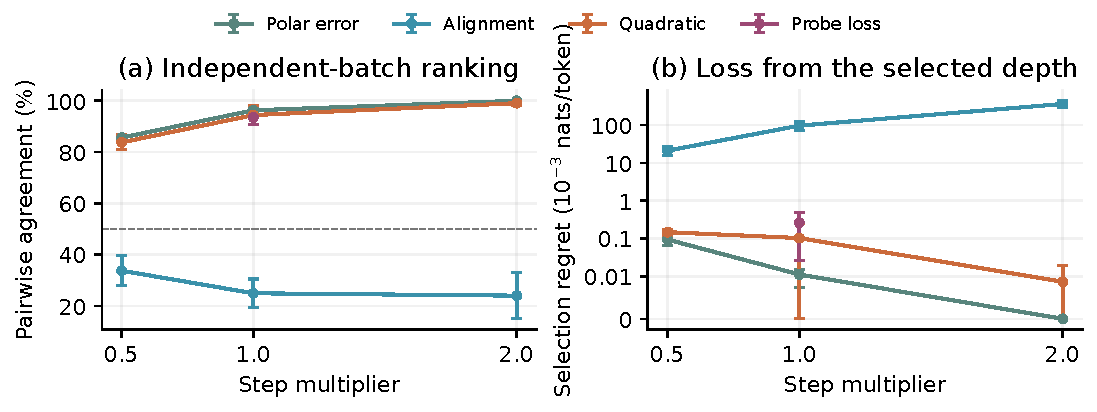
\includegraphics[width=\linewidth]{figures_v2/v2_probe_ranking.pdf}
\caption{独立批次上各选择依据的排序一致率与选择损失。误差条为训练种子间的一个样本标准差。
右图在零附近使用线性刻度，其余使用对数刻度。}
\label{fig:v2ranking}
\end{figure}

精确极因子也沿共同RMS生成完整步长。
在实际步长下，NS5与精确极因子的平均损失下降分别为$5.73\times10^{-4}$和$3.57\times10^{-4}$ nats/token。
72个配对测量中，NS5下降更多的有50个，精确极因子下降更多的有21个，另外1个在$10^{-7}$内并列。
在WikiText103冻结状态中，四类隐藏矩阵的归一化稳定秩随深度上升。
从NS1到NS5，小模型的平均值由0.018增至0.564，大模型由0.013增至0.569。
在相同总能量下，较深的候选把更新能量分配到更多奇异方向，见附录图\ref{fig:v2spectra}。

\subsection{固定深度在匹配训练中的收益}
在WikiText103的26.5M参数模型上，NS1、NS3和NS5使用相同的矩阵峰值学习率0.003，
每个隐藏矩阵的非衰减更新均具有相同的RMS。
三组的终点验证损失依次为5.5799、4.8954和4.8118 nats/token。
NS5相对NS3将终点验证损失平均降低0.0836，将测试损失平均降低0.0847。
三个配对种子上的两种损失均保持这一排序。
在这一配置中，增加深度改善了训练，同状态探测表明较浅方向经常承担更高的二阶代价。

AdamW经过相同规则的学习率筛选，终点验证损失为5.1240。
幅度匹配动量在独立选定的峰值学习率下取得5.3293。
表\ref{tab:v2main}列出各方法的学习率、终点验证损失和验证所选检查点的测试损失。
NS深度效应来自共同步长与共同辅助参数的配对对照。

\begin{table}[htbp]\centering\small
\caption{WikiText103的26.5M参数模型。每种方法使用三个配对种子，表中为均值和一个样本标准差。损失单位为nats/token。}
\label{tab:v2main}
\input{v2_table_main}
\end{table}

\input{v2_training_extended}



\FloatBarrier
\section{结论}
有限步正交化重分配矩阵更新在不同奇异方向上的能量，改变参数步长承担的曲率代价。给定相同梯度、动量和Hessian谱，
只需交换低曲率方向，就能改变线优化后的最优深度。二维相图给出了这一变化随梯度比和曲率比移动的精确分界。
对实际训练步长，方向曲率解释了采用较少迭代的候选为何会失去较高的一阶收益。
极因子误差此时也能准确排序，减小步长后则有更多状态由较浅候选取得最大下降。

在等幅训练中，三步增至五步带来的收益延续到较长训练。目标反馈的深度选择集中于NS5，
固定NS5在三组语言模型对照中取得较低的平均测试损失。
在实测步长下，低谱误差候选反复占优，在线探测多次返回同一个深度。
对发生切换的两条轨迹，采用NS3的时机解释了反馈与固定深度之间的大部分测试损失差距。

\paragraph{代码与数据。}
实验入口、冻结配置和生成图表的命令见
\href{https://github.com/Higgsfield-DHY/optimization-course-muon/tree/course-v2.0}{实验代码与复现材料（course-v2.0）}。
\bibliographystyle{unsrtnat}
\bibliography{references}
\appendix
\section{有限深度驻点界的证明}\label{app:v2convergence}
记$\tau_\ell$为动量的Frobenius范数，$M_\ell$的奇异值为$\sigma_{\ell,i}$。
对非零块，令$s_i=\sigma_{\ell,i}/\tau_\ell$。谱变换和幅度匹配给出
\[
 \inner{M_\ell}{D_\ell}
   = R_\ell\tau_\ell\frac{\sum_i s_i q_k(s_i)}
                      {(\sum_i q_k(s_i)^2)^{1/2}}
   \ \ge\ \alpha R_\ell\norm{M_\ell}_F .
\]
零动量块的两端均为零。记$e=M-g$，应用三角不等式及Cauchy--Schwarz不等式，
\begin{align}
 \inner{g}{D}
 &\ge \alpha\sum_\ell R_\ell\norm{g_\ell}_F
        -(1+\alpha)\sum_\ell R_\ell\norm{e_\ell}_F\\
 &\ge C\norm{g}-(1+\alpha)S\norm{e}.
\end{align}
$\norm{D}\le S$且$0\le\eta\lambda\le1/(2T)$，
因而$\norm{w_t}\le\norm{w_0}+\eta St$，$\lambda\norm{w_t}\le C/2$。
令$H_t=D_t+\lambda w_t$，可得
$\norm{H_t}\le S'$和
$\inner{g_t}{H_t}\ge(C/2)\norm{g_t}-(1+\alpha)S\norm{e_t}$。
光滑性给出
\[
 f(w_{t+1})\le f(w_t)-\eta\inner{g_t}{H_t}
                    +(L_f\eta^2/2)(S')^2 .
\]

展开动量递推。令$\zeta_i=G_i-g_i$，得到
\begin{align}
 e_t&=-\beta^{t+2}g_0-\sum_{i=1}^{t}\beta^{t-i+2}(g_i-g_{i-1})+N_t,\\
 N_t&=(1-\beta)\sum_{i=0}^{t-1}\beta^{t-i+1}\zeta_i
                     +(1-\beta^2)\zeta_t .
\end{align}
历史条件无偏性使噪声的交叉项期望为零，并给出
\[
 \mathbb E\norm{N_t}^2
 \le \sigma^2\left[\frac{(1-\beta)^2}{1-\beta^2}+(1-\beta^2)^2\right]
 \le 3\sigma^2(1-\beta).
\]
第二个不等号使用$(1-\beta)^2/(1-\beta^2)\le1-\beta$和
$(1-\beta^2)^2\le2(1-\beta)$。
梯度漂移每步至多为$L_f\eta S'$。
对初始化项和漂移项各求一次几何和，得到
\[
 \frac1T\sum_{t=0}^{T-1}\mathbb E\norm{e_t}
 \le \frac{\norm{g_0}}{T(1-\beta)}
       +\frac{L_f\eta S'}{1-\beta}
       +\sigma\sqrt{3(1-\beta)}.
\]
在下降不等式中代入此式，对迭代求和并使用$f(w_T)\ge f_*$，
即得定理\ref{thm:v2convergence}。

\section{补充实验与复现}
\subsection{矩阵轨迹}
训练前在独立种子101上比较各候选的峰值学习率，选择500步后的最小目标值。
正式种子0至9共享初始目标值1，匹配优化器使用的随机噪声序列。
每10步记录真梯度范数与目标值。图\ref{fig:v2trajectory}按种子计算均值和样本标准差。

\begin{figure}[htbp]\centering
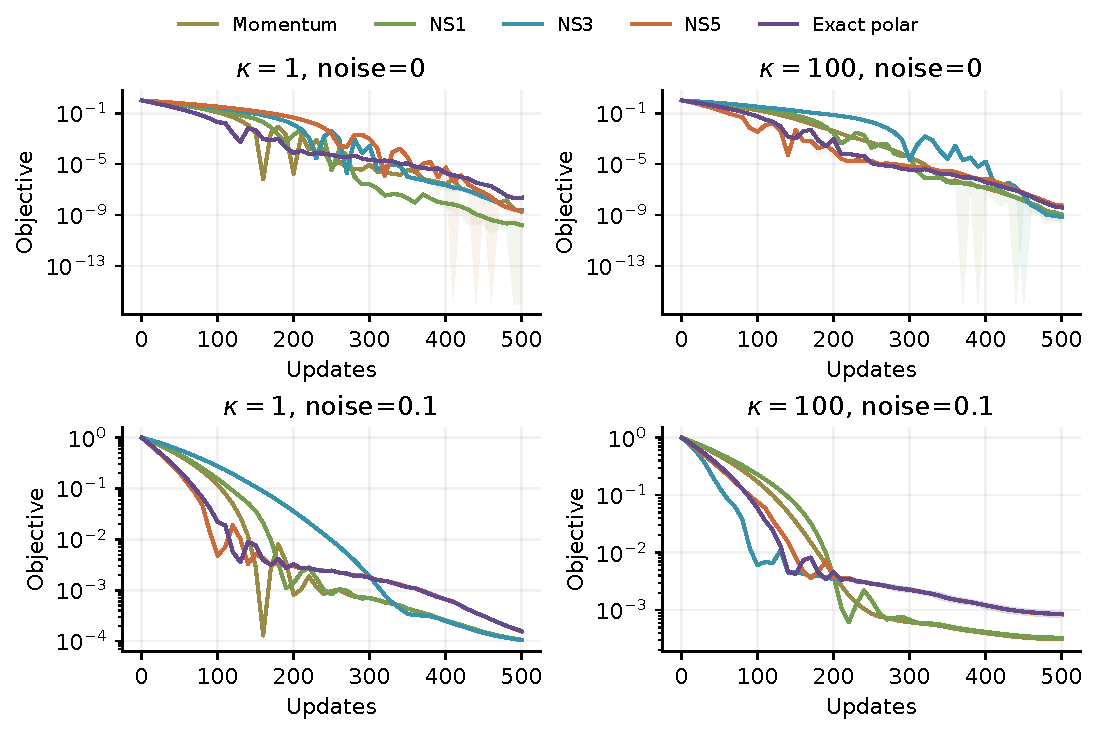
\includegraphics[width=\linewidth]{figures_v2/v2_matrix_trajectories.pdf}
\caption{倒置曲率的矩阵优化轨迹。横轴为更新步数，纵轴为目标值，阴影为10个种子的一个样本标准差。}
\label{fig:v2trajectory}
\end{figure}

\subsection{验证、测试与冻结更新}
WikiText103的验证集与测试集分别有251048和287644个预测目标。
TinyStories的验证使用固定的262144个目标，测试共2369481个目标。
数据按连续token分块，尾块只累计实际目标。
种子配对使用完整的同一训练步数。测试分数取该种子在验证损失最低点保存的模型。

在主实验的NS5与Probe-NS、较大模型的NS5、TinyStories的NS5四组中，
每种子保存3个更新前状态，共36个锚点。
每个锚点保存基础参数、训练动量、候选全量更新和数据身份。
从实际存档步长中扣除权重衰减后，隐藏矩阵方向RMS与目标0.2的最大差为$4.59\times 10^{-8}$。
谱统计使用首层融合QKV、中层MLP上投影、末层注意力输出和MLP下投影四个矩阵。
局部曲率和完整步长响应使用float32计算。

\begin{figure}[htbp]\centering
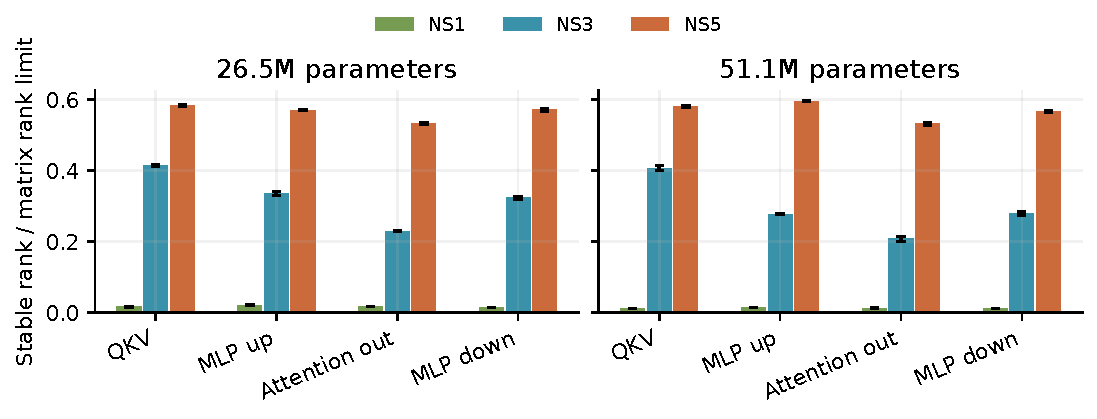
\includegraphics[width=\linewidth]{figures_v2/v2_update_spectra.pdf}
\caption{WikiText103中实际候选更新的谱形状。稳定秩除以矩阵的最大可能秩。
每个种子内先在锚点上平均，误差条为三个种子的样本标准差。}
\label{fig:v2spectra}
\end{figure}

\subsection{重放深度与实际干预长度}
表\ref{tab:v2replay}给出每个种子的探测选择与重放序列。
第100、200、\ldots、1000步发生选择。末次选择只作用于第1000步，重放固定该位置。
表的最后一列把不同的选择换算成实际采用不同深度的更新数。
\begin{table}[htbp]\centering
\caption{目标反馈和阶段匹配重放的逐种子选择。}
\label{tab:v2replay}
\begin{tabular}{cllr}
\toprule
种子 & Probe-NS深度 & 重放深度 & 改动步数 \\ \midrule
0 & 5,5,5,5,5,5,5,5,5,5 & 5,5,5,5,5,5,5,5,5,5 & 0 \\
1 & 5,5,5,5,5,5,5,5,3,5 & 5,5,5,5,5,5,5,5,3,5 & 0 \\
2 & 5,5,5,5,5,5,5,5,3,5 & 5,5,5,5,5,5,5,5,3,5 & 0 \\
\bottomrule
\end{tabular}

\end{table}

\end{document}
